%%---------------------------------------------------------------------------%%
\section{NekRS: recent developments enabling large scale ExaSMR simulations}
\label{sec:nekrs}

NBekRS is a new GPU-oriented version of Nek5000  that is also capable of running
on CPUs. It represents a significant redesign of the code. While written in
C++, NekRS is able to link to Nek5000 to leverage its extensive pre- and
postprocessing utilities. NekRS relies on a native GPU library,
libParanumal \cite{libP}, for highly-performant kernels to evaluate (and
solve) the PDE operators.  The main kernels require fast evaluation of the
Laplacian (for the viscous Helmholtz solves for each velocity component and
for the pressure-Poisson solve), fast preconditioners (for pressure), and
fast, fully dealiased, advection operators.  The coarse-grid pressure solves
are performed with Hypre.

\subsection{Performance Improvements}

Over the past year there have been several performance improvements in NekRS. These improvements enabled the significant increase in performance measured here.
A few of the most important improvements are:
\begin{itemize}
  \item New GPU-aware gather-scatter routines;
  \item Improved Pressure-Poisson precondtioner;  
  \item Support for Half-precision in the preconditioner;
  \item Addition of residual projection.
\end{itemize}
Details on these improvements are to be discussed in an upcoming paper and CEED report.

\subsection{Stability-Enhanced Wall-Resolved Models: $k-\tau$}
Another significant development during the past year was the implementation of the $k-\tau$
version of the $k-\omega$ model and the investigation of the scaling of all the terms appearing in
the right-hand-side of the $k$ and $\tau$ equations. The model has been implemented in both Nek5000 and NekRS. The $k-\tau$ model was originally developed by Benton et al.~\cite{benton1996application} as an alternative
implementation of the $k-\omega$ model. The equations for $k$ and $\tau$ are derived from the $k-\omega$
equations by using the definition $\tau=1/\omega$:

\begin{equation}
    \frac{\partial (\rho k)}{\partial t} + \nabla\cdot(\rho k \bf{v}) =  \nabla\cdot\left[(\mu+\frac{\mu_t}{\sigma_k})\nabla k\right] + P-\rho \beta^{*}\frac{k}{\tau}
\end{equation}

\begin{equation}
 \frac{\partial (\rho \tau)}{\partial t} + \nabla\cdot(\rho\tau \bf{v}) =  \nabla\cdot\left[(\mu+\frac{\mu_t}{\sigma_\omega })\nabla \tau \right] - \gamma \frac{\tau}{k} P+\rho \beta-2\frac{\mu}{\tau}\left(\nabla\tau\cdot\nabla\tau\right)
\end{equation}

where now $G_k=P$, $Y_k=\beta^{*}k/\tau$, $G_\tau=\gamma\tau P/k$, $Y_\tau=\beta$ and $S_\tau=2\nu\left(\nabla\tau\cdot\nabla\tau\right)/\tau$.

In contrast to the original form of the $k-\omega$ model, in which the $\omega$ equation contains
terms that become singular close to  wall boundaries, all terms in the right-hand side of the $k$ and $\tau$ equations reach a finite  limit at walls and do not need to be treated  asymptotically; that is, they do not require regularization for numerical implementation. The Nek5000 version of  $k-\tau$ has been benchmarked extensively across a variety of canonical cases including channel flow and the backward facing step. The NekRS version has been tested against channel flow. We discuss in the following a more extensive verification study for rod bundles.

\subsection{Verification of the $\lowercase{k}-\tau$ RANS model in NekRS}
\label{sec:nrs1}
The $k-\tau$ model is implemented in nekRS as the primary RANS model because of two important reasons: (i) its capability in predicting the wall-bounded turbulent flows, and (ii) the relatively easier treatment of boundary conditions. Before conducting the large-scale full core CFD simulations with nekRS, a verification study is performed to ensure the $k-\tau$ model implemented in nekRS produces consistent results as in its CPU-only version, Nek5000. A 2x2 subchannel bundle domain is selected in the testing case. Identical boundary and initial conditions are specified in the nekRS and Nek5000 test cases. The same set of input parameters are given in both cases, such as the time step size, residual tolerances, etc. The cases are run long enough till the steady state. Figure~\ref{fig:tkeofbundle} shows the turbulent kinetic energy distribution under the steady state. A quantitative comparison is presneted in Figure~\ref{fig:tkeplot} and Figure~\ref{fig:tauplot} where the nekRS was able to reproduce the exact solutions of Nek5000. This benchmark study provides a strong footing as we move on to the more extensive  verification and applications of $k-\tau$ model in nekRS.

\begin{figure}[!ht]
\centering
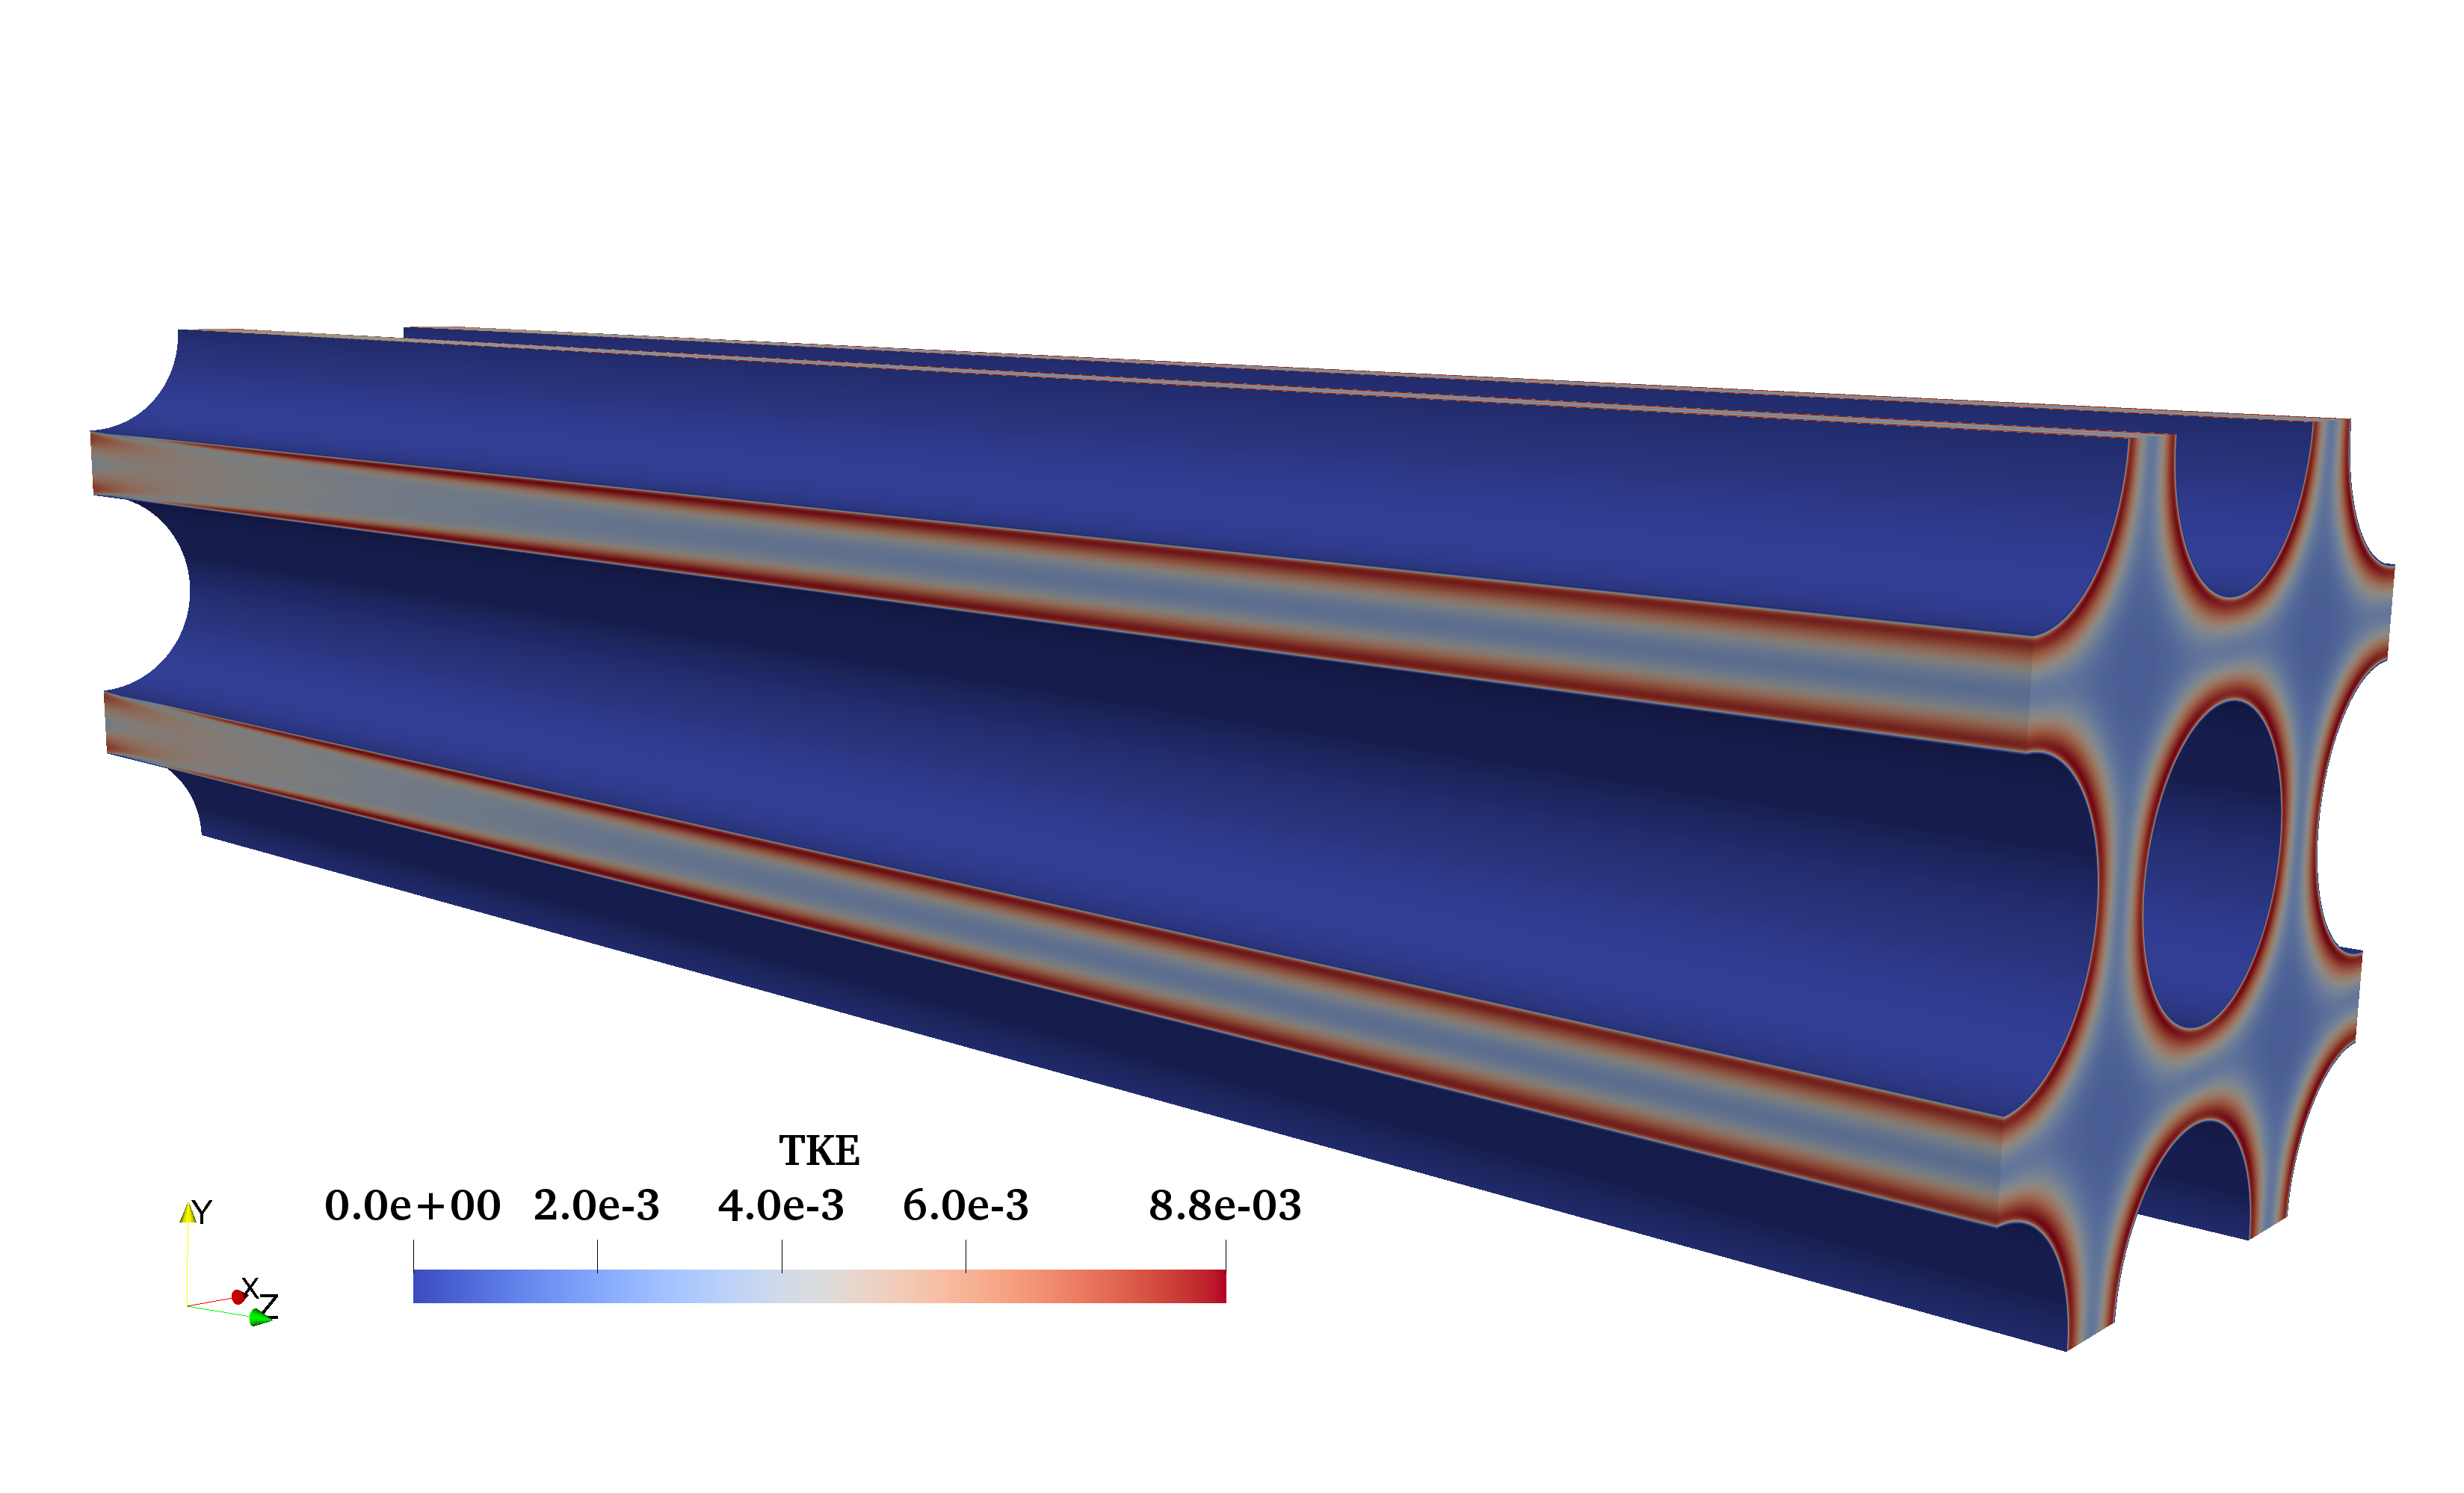
\includegraphics[width=0.5\textwidth]{./figures/TKE_in_bundle.png}
\caption{The steady-state turbulent kinetic energy distribution in the nekRS test case. }
\label{fig:tkeofbundle}
\end{figure}

\begin{figure}[!ht]
\centering
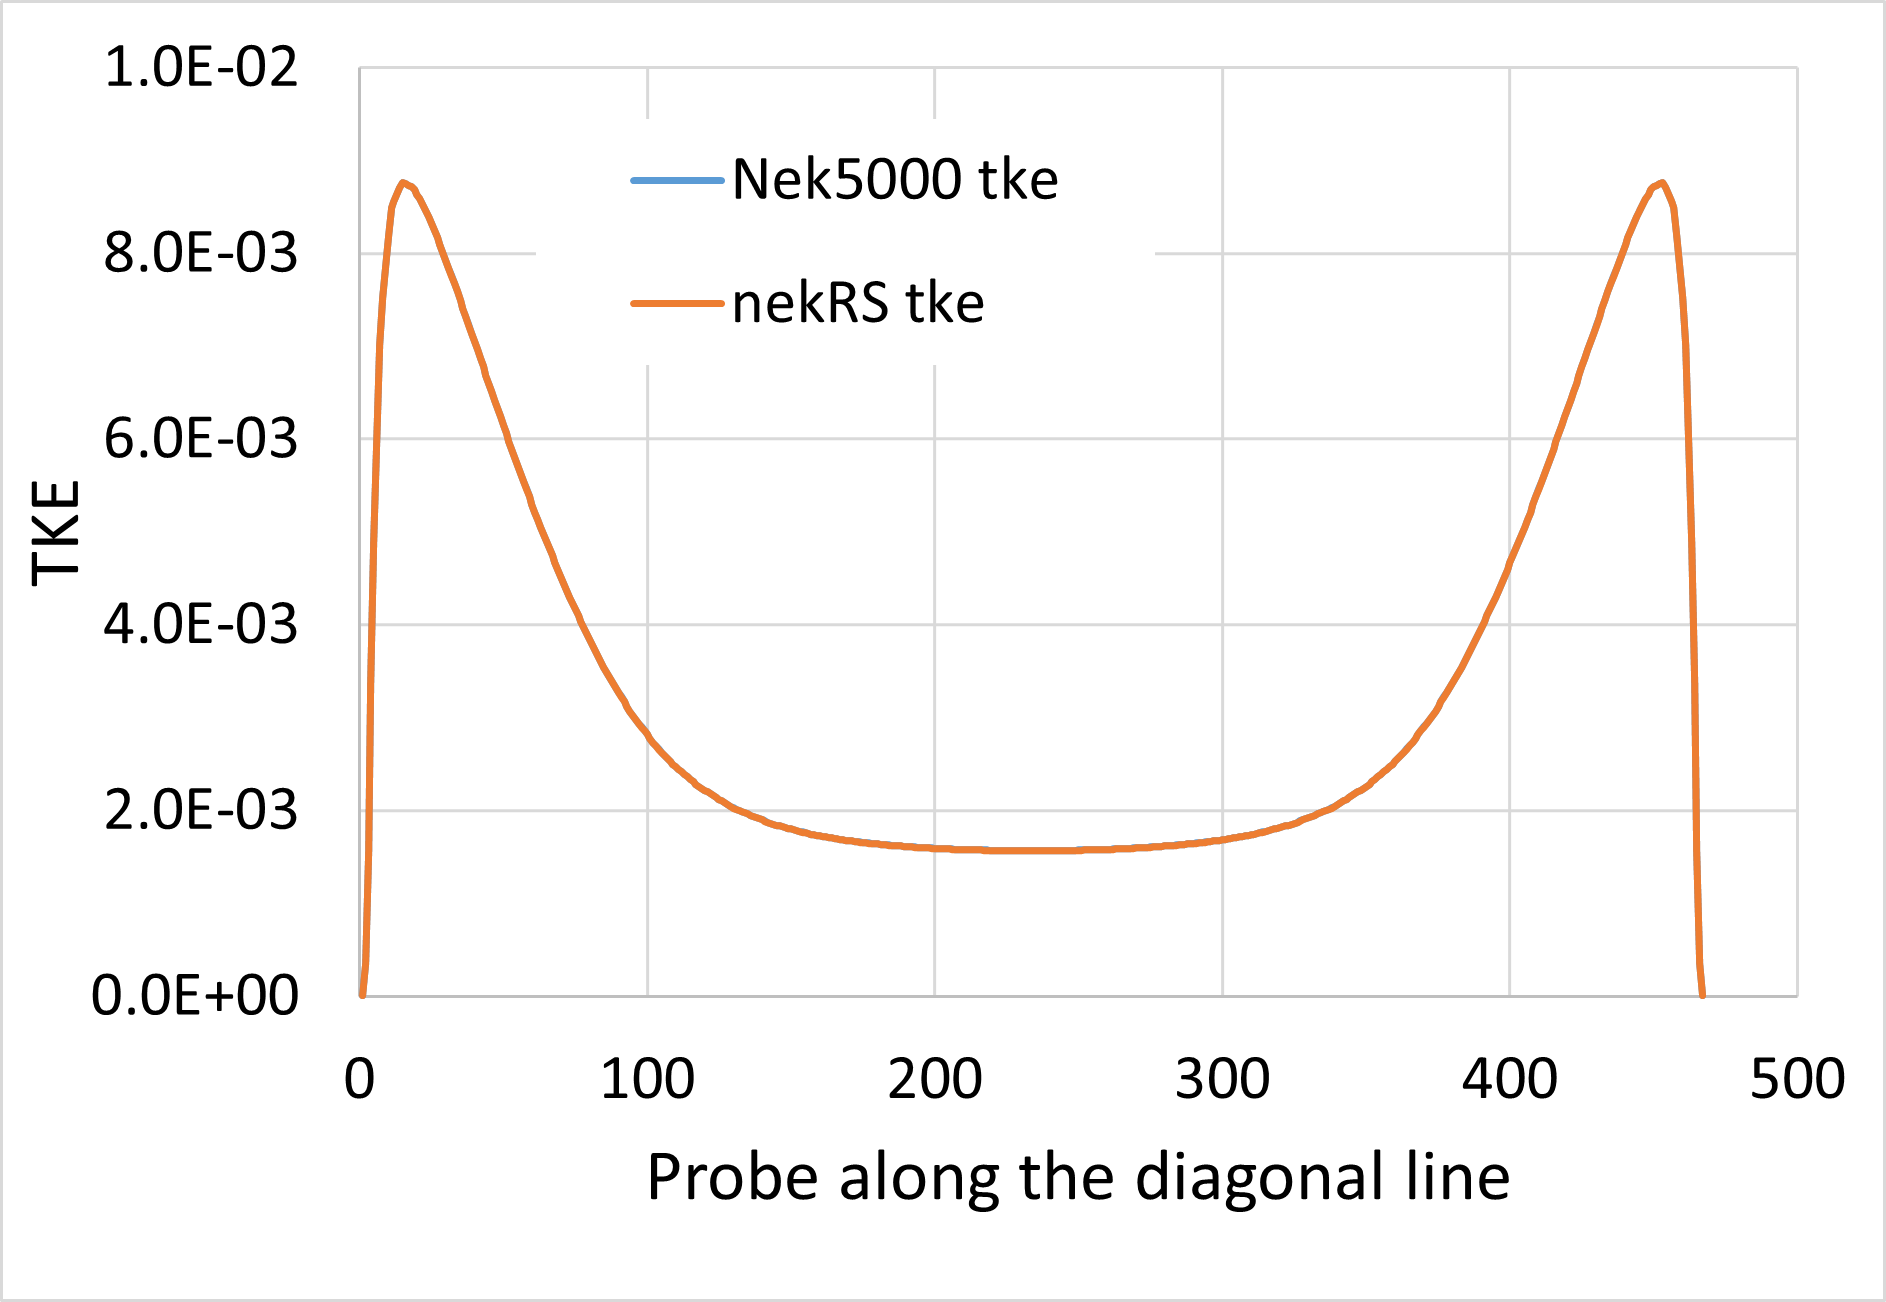
\includegraphics[width=0.5\textwidth]{./figures/tke_verification_bundle2x2.png}
\caption{Comparison of $k$ profile along the outlet diagonal line from Nek5000 and nekRS tests. }
\label{fig:tkeplot}
\end{figure}

\begin{figure}[!ht]
\centering
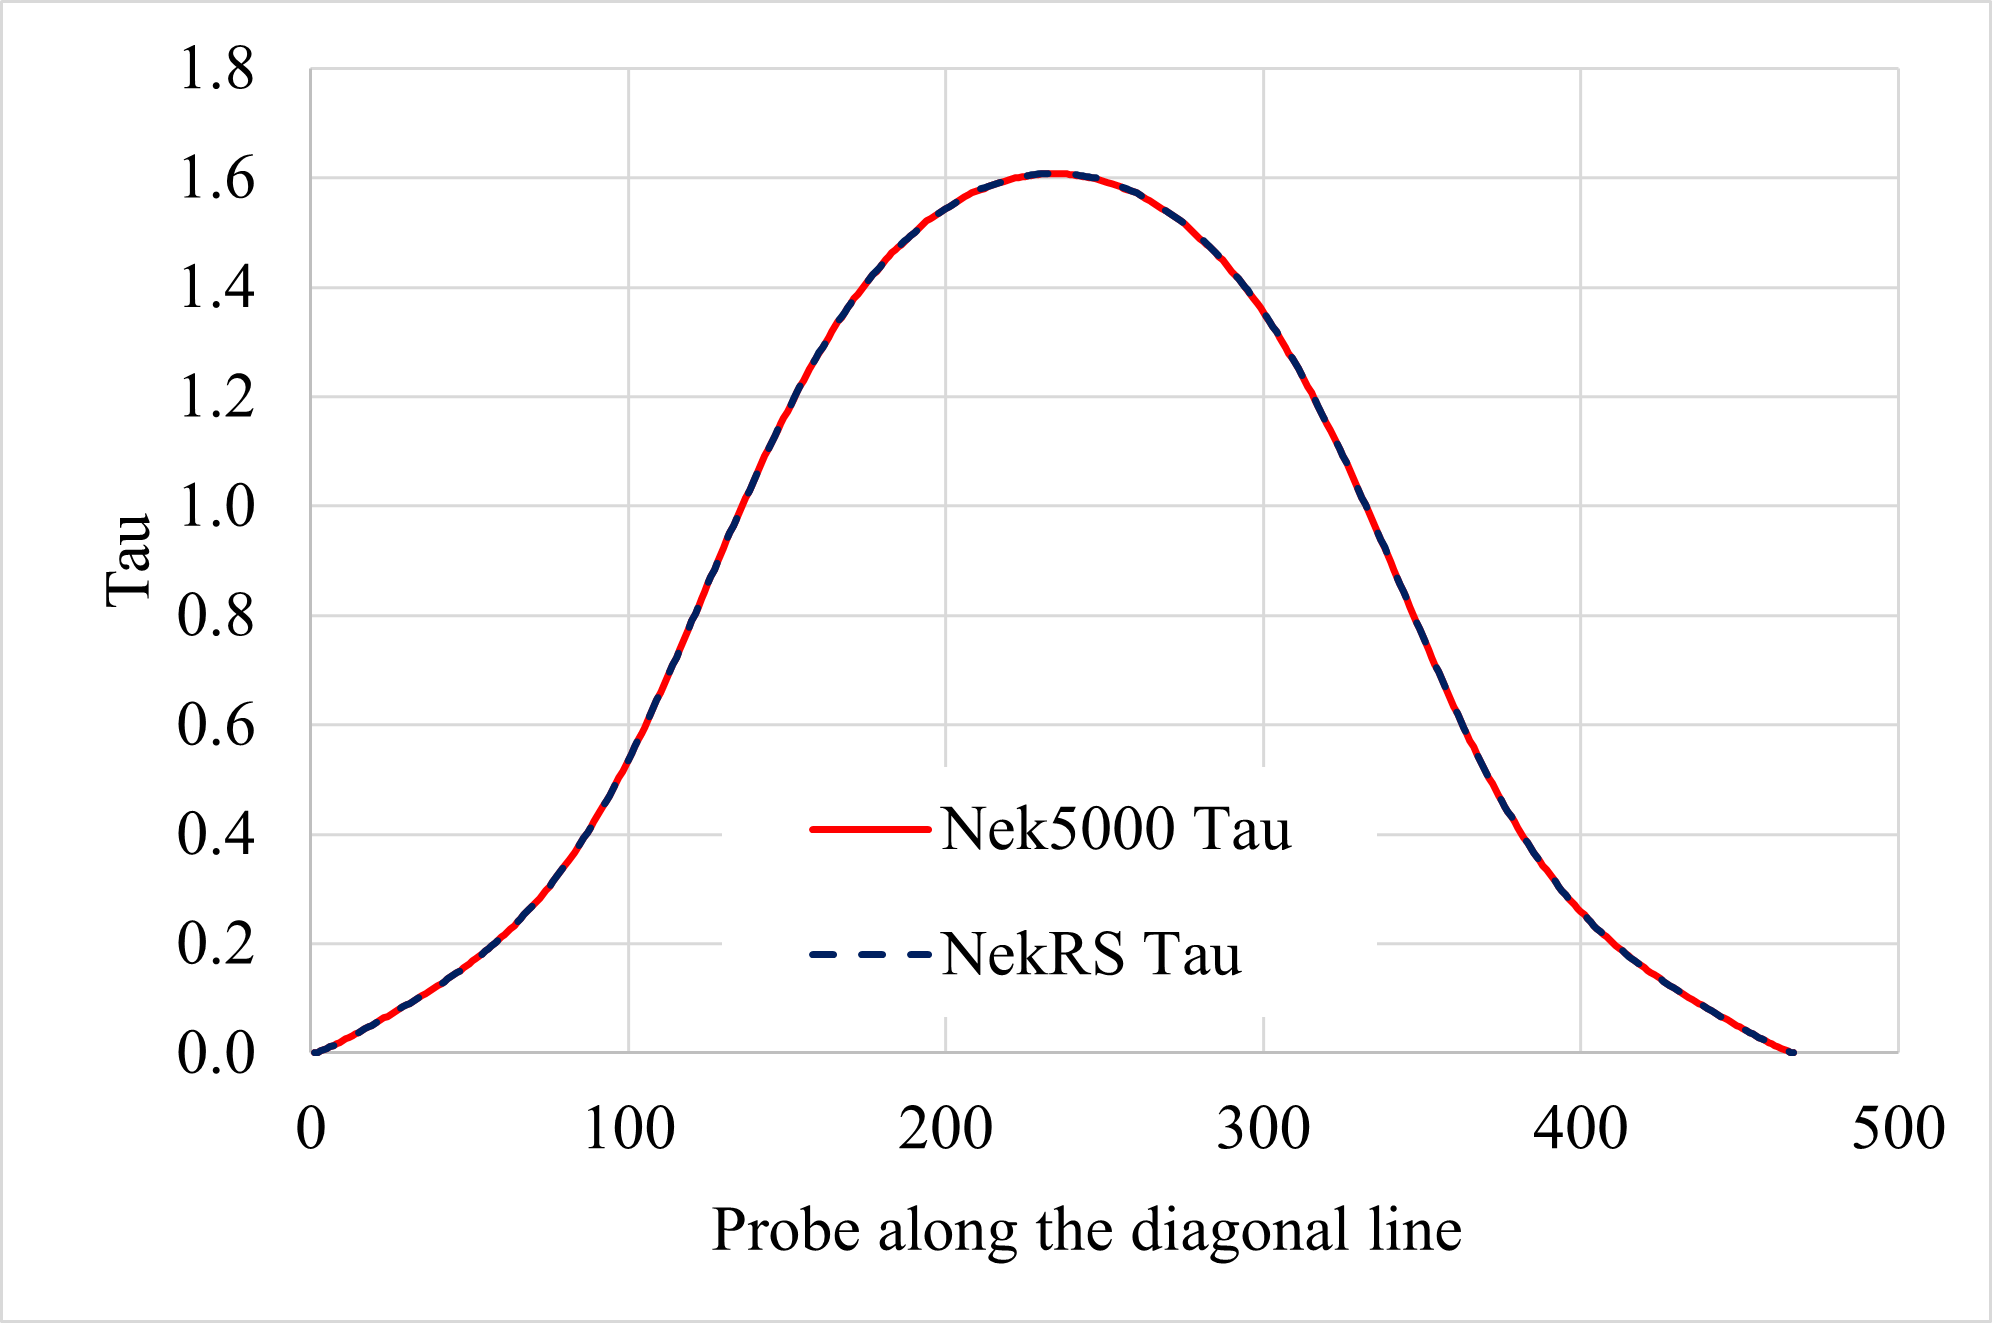
\includegraphics[width=0.5\textwidth]{./figures/tau_verification_bundle2x2.png}
\caption{Comparison of $\tau$ profile along the outlet diagonal line from Nek5000 and nekRS tests. }
\label{fig:tauplot}
\end{figure}
